\section*{Lezione 10}
\addcontentsline{toc}{section}{Lezione 10}

\subsection*{Sorgente Bernoulliana}
\addcontentsline{toc}{subsection}{Sorgente Bernoulliana}

Data una sorgente $S=\{s_1, s_2\}$ in cui $s_1$ ha probabilità $p$ e $s_2$ ha probabilità $1-p$, la sua entropia vale

\begin{equation*}
H_2(p) = p\log_2\frac{1}{p} + (1-p)log_2\frac{1}{1-p}
\end{equation*}

Questa è una funzione a una variabile (e non due). In generale $H_r(p_1, p_2, ..., p_q)$ è una funzione a $q-1$ variabili.
Proviamo a disegnare la funzione entropia della sorgente Bernoulliana:


\begin{figure}[h]
	\centering
	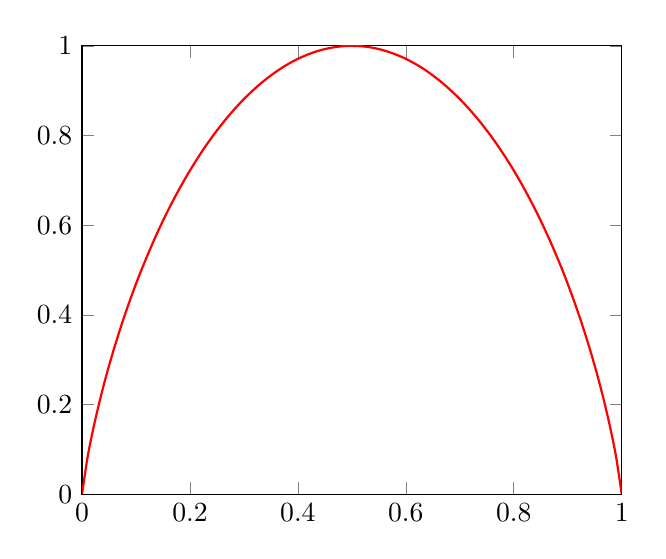
\begin{tikzpicture}
	\begin{axis}[
	xmin = 0, xmax = 1,
	ymin = 0, ymax = 1,
	]
	\addplot[
	domain = 0:1,
	samples = 100,
	smooth,
	thick,
	red,
	] {x*log2(1/x) + (1-x)*log2(1/(1-x))};
	\end{axis}
	\end{tikzpicture}
	\caption{Grafico sorgente Bernoulliana}
\end{figure}

Sembra una parabola ma non lo è (in 0 la derivata ha pendenza infinita).
Il valore massimo (1) si ottiene per $p=\frac{1}{2}$, il minimo (0) quando $p=0 \lor p=1$.
Dove si trova invece il valore massimo per il caso generale $H_r(p_1, p_2, ..., p_q)$?

\newpage

\subsection*{Disuguaglianza di Gibbs}
\addcontentsline{toc}{subsection}{Disuguaglianza di Gibbs}

\begin{figure}[h]
	\centering
	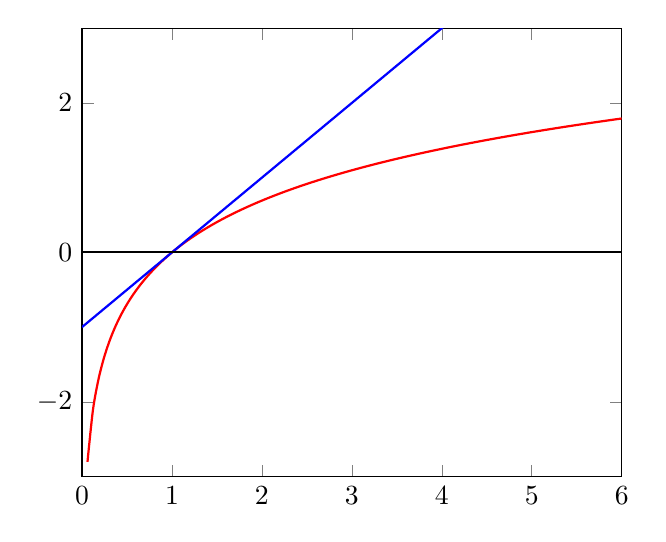
\begin{tikzpicture}
	\begin{axis}[
	xmin = 0, xmax = 6,
	ymin = -3, ymax = 3,
	]
	\addplot[
	domain = 0:6,
	samples = 100,
	smooth,
	thick,
	red,
	] {ln(x)};
		\addplot[
	domain = 0:6,
	samples = 100,
	smooth,
	thick,
	blue,
	] {x-1};
	] {ln(x)};
	\addplot[
	domain = 0:6,
	samples = 2,
	smooth,
	thick,
	black,
	] {0};
	\end{axis}
	\end{tikzpicture}
	\caption{Grafico $y=x-1$ (in blu) e $y=ln(x)$ (in rosso)}
\end{figure}

Notiamo che $ln(x) <= x - 1 \; \; \forall x > 0$ e vale $ln(x) = x$ se $x = 1$.

Prendiamo due distribuzioni di probabilità
\begin{equation*}
x_1, x_2, ... , x_q
\end{equation*}
\begin{equation*}
y_1, y_2, ... , y_q
\end{equation*}
La disuguaglianza di Gibbs ci dice che:
\begin{empheq}[box=\tcbhighmath]{equation*}
\sum_{i=1}^qx_i\log_2(\frac{y_i}{x_i}) \leq 0
\end{empheq}

\textbf{Dimostrazione non richiesta all'orale}, però la scrivo dai

\begin{dimostrazione}
	Partiamo da:
	\begin{equation*}
	\sum_{i=1}^qx_i\log_2(\frac{y_i}{x_i}) = \frac{1}{\ln2}\sum_{i=1}^qx_i\ln(\frac{y_i}{x_i})
	\end{equation*}
	Ora sfruttiamo la maggiorazione di prima:
	\begin{equation*}
    \frac{1}{\ln2}\sum_{i=1}^qx_i\ln(\frac{y_i}{x_i}) \leq \frac{1}{\ln2}\sum_{i=1}^qx_i(\frac{y_i}{x_i} - 1)
	\end{equation*}
		\begin{equation*}
	\frac{1}{\ln2}\sum_{i=1}^qx_i\ln(\frac{y_i}{x_i}) \leq \frac{1}{\ln2}\sum_{i=1}^q(y_i-x_i)
	\end{equation*}
		\begin{equation*}
	\frac{1}{\ln2}\sum_{i=1}^qx_i\ln(\frac{y_i}{x_i}) \leq \frac{1}{\ln2}[\sum_{i=1}^qy_i-\sum_{i=1}^qx_i]
	\end{equation*}
	Ma essendo le due sommatorie $\sum_{i=1}^qy_i-\sum_{i=1}^qx_i$ e $\sum_{i=1}^qy_i-\sum_{i=1}^qx_i$ sono uguali a 1, allora:
			\begin{equation*}
	\frac{1}{\ln2}\sum_{i=1}^qx_i\ln(\frac{y_i}{x_i}) \leq \frac{1}{\ln2}[0-0]
	\end{equation*}
	\begin{equation*}
	\sum_{i=1}^qx_i\ln(\frac{y_i}{x_i}) \leq 0
	\end{equation*}
	Questo funziona solo se $x_i = y_i$ per tutte le $i$, quindi se e solo se le due distribuzioni di probabilità sono uguali.
\end{dimostrazione}

Ora possiamo usare la disuguaglianza per trovare il valore massimo dell'entropia.

Calcoliamo

\begin{equation*}
H_2(S)-\log_2q = \sum_{i=1}^qp_ilog_2\frac{1}{p_i} - (log_2q)\sum_{i=1}^qp_i
\end{equation*}
\begin{equation*}
= \sum_{i=1}^qp_i[\log_2\frac{1}{p_i} - \log_2q] = \sum_{i=1}^qp_i\log_2\frac{1}{p_iq} = \sum_{i=1}^qp_i\log_2\frac{\frac{1}{q}}{p_i}
\end{equation*}
Applico Gibbs e scopro che:
\begin{equation*}
 \sum_{i=1}^qp_i\log_2\frac{\frac{1}{q}}{p_i} \leq 0
\end{equation*}
E quindi:
\begin{equation*}
H_2(S) \leq \log_2q
\end{equation*}
e l'entropia raggiunge il valore massimo (quindi $\log_2q$) solo quando i valori di probabilità sono uguali, quindi quando la distribuzione è uniforme.

Quindi l'entropia $H_2(S)$:
\begin{itemize}
	\item \'E sempre maggiore o uguale di zero, in particolare è $=0$ quando la distribuzione di probabilità assegna ad una $p_i$ valore 1 e al resto valore 0
	\item \' E sempre minore o uguale a $\log_2q$, e raggiunge questo valore massimo quando la distribuzione di probabilità è uniforme.
\end{itemize}

Ora supponiamo di avere una sorgente $S=\{s_1, s_2, ..., s_q\}$ che codifica un codice istantaneo $r$-ario con codeword di lunghezza $\ell_1, \ell_2, ..., \ell_q$.
Proviamo a mettere in relazione la lunghezza media con l'entropia della sorgente.
Essendo il codice istantaneo vale la disuguaglianza di Kraft:
\begin{equation*}
\sum_{i=1}^q\frac{1}{r^{\ell_i}} \leq 1
\end{equation*}

Ora definiamo per $i=1,2,...q$ 
\begin{equation*}
Q_i = \frac{r^{-\ell_i}}{K}
\end{equation*}

che sarebbe uno dei termini della somma fratto la somma totale

\begin{equation*}
0 \leq Q_i = \frac{r^{-\ell_i}}{K} \leq 1
\end{equation*}

Posso dire che

\begin{equation*}
\{Q_1, Q_2, ..., Q_q\}
\end{equation*}
è una distribuzione di probabilità, e vale $\sum_{i=1}^qQ_i = 1$.
(P.S. questo conto qua non serve orale)

Ora uso queste due distribuzioni per scrivere la disuguaglianza di Gibbs

\begin{equation*}
\sum_{i=0}^qp_i\log_2\frac{Q_i}{p_i} \leq 0
\end{equation*}

Ora lavoriamoci su:

\begin{equation*}
\sum_{i=0}^qp_i\log_2\frac{Q_i}{p_i} =
\end{equation*}
\begin{equation*}
= \highlight{\sum_{i=0}^qp_i[\log_2\frac{1}{p_i}} - \log_2\frac{1}{Q_i}]
\end{equation*}
\begin{equation*}
= H_2(S) - \sum_{i=0}^qp_i\log_2\frac{1}{Q_i} \leq 0
\end{equation*}
\begin{equation*}
= H_2(S) \leq \sum_{i=0}^qp_i\log_2\frac{1}{Q_i}
\end{equation*}
\begin{equation*}
= H_2(S) \leq \sum_{i=0}^qp_i\log_2\frac{K}{r^{-\ell_i}}
\end{equation*}
\begin{equation*}
= H_2(S) \leq \sum_{i=0}^qp_i[\log_2K - \log_2{r^{-\ell_i}}]
\end{equation*}
\begin{equation*}
= H_2(S) \leq \log_2K \sum_{i=0}^qp_i + \log_2{r^{-\ell_i}}
\end{equation*}
\begin{equation*}
= H_2(S) \leq \log_2K \sum_{i=0}^qp_i + \log_2r\sum_{i=1}^qp_i\ell_i
\end{equation*}
\begin{equation*}
= H_2(S) \leq \log_2K + \log_2r \cdot L
\end{equation*}

Noto che $K \leq 1$, quindi il logaritmo di un valore minore di 1 è $\leq 0$, quindi posso minorare ulteriormente

\begin{equation*}
= H_2(S) \leq \log_2r \cdot L
\end{equation*}

Riscrivo tutto come:

\begin{equation*}
\frac{1}{\log_2r} \cdot H_2(S) \leq L
\end{equation*}
La quantità $\frac{1}{\log_2r}$ fa un cambio di base nel logaritmo dell'entropia, quindi:

\begin{empheq}[box=\tcbhighmath]{equation*}
H_r(S) \leq L
\end{empheq}

Questa disuguaglianza mi dice che data una sorgente $S$ istantanea con una lunghezza media $L$, essa non può essere più piccola dell'entropia misurata in base $r$.
Quindi la lunghezza media non può essere più piccola dell'entropia.\\
Quando rappresento in maniera compatta è come se le stessi comprimendo delle sequenze, se scendo sotto una certa soglia vuol dire che sto perdendo informazione. Quindi l'entropia rappresenta anche una soglia minima per quanto riguarda la lunghezza media delle codeword.\\
In pratica più mi avvicino all'entropia più sto comprimendo la lunghezza media.

\medskip
La seguente disuguaglianza vale anche per i codici univocamente decodificabili (thanks McMillan) visto che la regola sulla $K$ vale anche su di essi.

\medskip

Quando però questa disuguaglianza diventa una uguaglianza (quindi ottengo la compressione massima)?

Nel passaggio da:

\begin{equation*}
= H_2(S) \leq \log_2K + \log_2r \cdot L
\end{equation*}

a

\begin{equation*}
= H_2(S) \leq \log_2r \cdot L
\end{equation*}

Dobbiamo fare in modo che $\log_2K$ sia uguale a 0, ovvero quando $K=1$. 

\subsection*{Codifica di Shannon-Fano}
\addcontentsline{toc}{subsection}{Codifica di Shannon-Fano}

Shannon e Fano partono da:

\begin{equation*}
H_r(S) \leq  L
\end{equation*}

che è un confronto fra medie (somma pesata vs somma pesata), ma vale la stessa cosa anche singolarmente?

\begin{equation*}
log_r\frac{1}{p_i} \leq \ell_i
\end{equation*}

Se fosse vero allora posso conoscere la lunghezza di una codeword a partire da $p_i$. Possiamo anche dire che $\ell_i$ è l'unico intero compreso in questo intervallo:

\begin{equation*}
log_r\frac{1}{p_i} \leq \ell_i < log_r\frac{1}{p_i} + 1
\end{equation*}

Chiamo queste lunghezze $\ell_i$ \textit{lunghezze di Shannon-Fano}.
Ma che tipo di codici ottengo con queste lunghezze? Codici istantanei; per dimostrarlo parto dalla disuguaglianza sopra (orale chiede):

\begin{equation*}
log_r\frac{1}{p_i} \leq \ell_i < log_r\frac{1}{p_i} + 1
\end{equation*}
\begin{equation*}
r^{log_r\frac{1}{p_i}} \leq r^{\ell_i} < r^{log_r\frac{1}{p_i} + 1}
\end{equation*}
\begin{equation*}
\frac{1}{p_i} \leq r^{\ell_i} < \frac{r}{p_i}
\end{equation*}
\begin{equation*}
p_i \geq \frac{1}{r^{\ell_i}} > \frac{p_i}{r}
\end{equation*}

Ora sommo tutte le $i$:
\begin{equation*}
\sum_{i=0}^qp_i \geq \sum_{i=0}^q\frac{1}{r^{\ell_i}} > \sum_{i=0}^qp_i\frac{1}{r}
\end{equation*}
\begin{equation*}
1\geq K > \frac{1}{r}
\end{equation*}

Quindi con queste lunghezze vale Kraft, quindi sono in grado di costruire un codice istantaneo.
La codifica di Shannon-Fano ci dice date le probabilità come sono definite le lunghezze, ma come trovo poi le codeword? Con l'albero di decodifica.

Ma allora perchè studiare Huffman? Esso ritorna un codice ottimale, vale anche per Shannon-Fano?

Siamo sicuri che 

\begin{equation*}
L_{\text{Huffman}} \leq L_{\text{Shannon-Fano}}
\end{equation*}

Andiamo a calcolare la lunghezza media di un codice creato tramite Shannon-Fano:

\begin{equation*}
log_r\frac{1}{p_i} \leq \ell_i < log_r\frac{1}{p_i} + 1
\end{equation*}
\begin{equation*}
p_i\log_r\frac{1}{p_i} \leq p_i\ell_i < p_i\log_r\frac{1}{p_i} + p_i
\end{equation*}
\begin{equation*}
\sum_{i=0}^qp_i\log_r\frac{1}{p_i} \leq \sum_{i=0}^qp_i\ell_i < \sum_{i=0}^qp_i\log_r\frac{1}{p_i} + \sum_{i=0}^qp_i
\end{equation*}
\begin{equation*}
H_r(S) \leq L_{Shannon-Fano} \leq H_r(S) + 1
\end{equation*}
E questo lo abbiamo già visto prima, però ci dice anche che non saranno mai più grandi di 1 dall'ottimo.
In pratica magari non saranno sempre ottimali, però nel caso non lo fossero non sono così tanto peggiori dell'ottimale.
In conclusione Huffman è più lento ma ottimale, Shannon Fano più veloce ma non sempre ottimale (ma non così male).

Vediamo un esempio di applicazione della codifica.

Sorgente con 6 simboli: $p_1 = p_2 = \frac{1}{4}$ $p_3 = p_4 = p_5 = p_6 = \frac{1}{8}$ con $r=2$.
Dobbiamo trovare il più piccolo $\ell_1$ tale per cui $log_2\frac{1}{p_i} \leq \ell_i$.

\begin{equation*}
\log_2\frac{1}{\frac{1}{4}} \leq \ell_1
\end{equation*}
\begin{equation*}
\log_24 \leq \ell_1
\end{equation*}
\begin{equation*}
2 \leq \ell_1
\end{equation*}
\begin{equation*}
\ell_1 = 2
\end{equation*}
\begin{equation*}
\ell_2 = 2
\end{equation*}

Quindi ho trovato le prime due.

\begin{equation*}
\log_2\frac{1}{\frac{1}{8}} \leq \ell_3
\end{equation*}
\begin{equation*}
\log_28 \leq \ell_3
\end{equation*}
\begin{equation*}
\ell_3 = 3
\end{equation*}
\begin{equation*}
\ell_4 = 3
\end{equation*}
\begin{equation*}
\ell_5 = 3
\end{equation*}
\begin{equation*}
\ell_6 = 3
\end{equation*}

Quindi costruisco l'albero a partire dalle lunghezze trovate:

\begin{figure}[H]
	\centering
	\vspace{4mm}
	\begin{tikzpicture}
	[
	grow                    = right,
	level 1/.style={sibling distance=8em},
	level 2/.style={sibling distance=5em},
	level 3/.style={sibling distance=2em},
	level distance          = 6em,
	edge from parent/.style = {draw, -latex},
	every node/.style       = {font=\footnotesize},
	sloped
	]
	\node [root] {}
	child { node [dummy] {}
		child { node [dummy] {}
			child { node [dummy] {$s_6$}
				edge from parent node [below] {0}}
			child { node [dummy] {$s_5$}
				edge from parent node [above] {1}}
			edge from parent node [above] {1}}
		child { node [dummy] {}
			child { node [dummy] {$s_4$}
				edge from parent node [below] {0}}
			child { node [dummy] {$s_3$}
				edge from parent node [above] {1}}
			edge from parent node [above] {0}}
		edge from parent node [above] {1}}
	child { node [dummy] {}
		child { node [dummy] {$s_2$}
			edge from parent node [above] {1}}
		child { node [dummy] {$s_1$}
			edge from parent node [above] {0}}
		edge from parent node [above] {0}}
	;
	\end{tikzpicture}
\end{figure}

\newpage
Vediamo ora un altro esempio basato su una sorgente Bernoulliana:

\begin{equation*}
p_1 = 1 - \frac{1}{2^k} \; \; \; \; \; \; \; (\text{n.b. k non è quella di kraft è un generico numero intero} > 1)
\end{equation*}

\begin{equation*}
p_2 = \frac{1}{2^k}
\end{equation*}

Huffman assegnerebbe 0 al primo simbolo e 1 al secondo simbolo, quindi $L_{\text{Huffman}} = 1$.

Vediamo ora la $L_{\text{Shannon-Fano}}$, quindi calcoliamo le lunghezze singole:

\begin{equation*}
\log_2\frac{1}{p_1} \leq \ell_1
\end{equation*}
Posso vedere $\frac{1}{p_1} = \frac{2^k}{2^k-1} = 1 + \frac{1}{2^k-1} \leq 2$
\begin{equation*}
\log_2\frac{1}{p_1} \leq \log_22
\end{equation*}
\begin{equation*}
\log_2\frac{1}{p_1} \leq 1 \leq \ell_1
\end{equation*}
\begin{equation*}
\ell_1 = 1
\end{equation*}

Ora la seconda:

\begin{equation*}
\log_2\frac{1}{p_2} = \log_22^k = k \leq \ell_2
\end{equation*}
\begin{equation*}
\ell_2 = k
\end{equation*}
\begin{equation*}
\ell_2 \geq 2
\end{equation*}
 
Ma se $k=1000$ allora ho la seconda codeword lunga 1000, vale ancora:
\begin{equation*}
H_r(S) \leq L_{Shannon-Fano} \leq H_r(S) + 1
\end{equation*}
\begin{center}
?
\end{center}
Sì certo perchè è una media pesata, quindi la seconda codeword la moltiplico per $\frac{1}{2^{1000}}$


\subsection*{Estensione di una sorgente}
\addcontentsline{toc}{subsection}{Estensione di una sorgente}

Ho una sorgente $S$ che emette i simboli $s_1, s_2, ..., s_q$ con probabilità $p_1, p_2, ..., p_q$.
Scelgo un numero $n \geq 1$ intero e definisco una nuova sorgente $S^n$ che chiamo $n$-sima estensione della sorgente $S$.\\
$S^n = S \times S ... \times S$\\
Gli elementi della sorgente $S^n$ sono quindi i simboli dell alfabeto, verranno chiamati $\sigma$ e $\sigma_i$ è l'$i$-esimo simbolo della sorgente $S^n$ è un vettore di $n$ elementi di $S$.
\begin{equation*}
\sigma_i=(S_{i1}, S_{i2}, ..., S_{in})
\end{equation*}
Dove per ogni componente ho $q$ possibilità. $q^n$ possibili simboli.
Quanto è la probabilità che esca $\sigma_i1$?
\begin{equation*}
p(\sigma_i) = p_{i1} \cdot p_{i2} \cdot ... \cdot p_{in}
\end{equation*}
Caso particolare è $n=1$, quindi vettori composti da un solo elemento ($\sigma_i = (s_1)$) e $q^1$ simboli.

\subsection*{Entropia in sorgenti estese}
\addcontentsline{toc}{subsection}{Entropia in sorgenti estese}
Quanto vale l'entropia di una sorgente $S^n$?
Chiamiamo $Q_i = p(\sigma_i) = p_{i1} \cdot p_{i2} \cdot ... \cdot p_{in}$.\\
Allora diciamo che:
\begin{equation*}
H_r(S^n) = \sum_{i=1}^{q^n}Q_i\log_r(\frac{1}{Q_i}) = \sum_{i=1}^{q^n}Q_i\log_r(\frac{1}{p_{i1} \cdot p_{i2} \cdot... \cdot p_{in}})
\end{equation*}
\begin{equation*}
= \sum_{i=1}^{q^n}Q_i\sum_{k=1}^n\log_r\frac{1}{p_{ik}}
\end{equation*}
\begin{equation*}
= \sum_{k=1}^{n}\sum_{i=1}^{q^k}(p_{i1} \cdot p_{i2} \cdot ... \cdot p_{in})\log_r\frac{1}{p_{ik}}
\end{equation*}
\begin{equation*}
...
\end{equation*}
\begin{equation*}
H_r(S^n) = n \cdot H_r(S)
\end{equation*}
L'ennesima estensione dell'entropia può essere vista come $n$ copie della sorgente che lavorano in parallelo:
\begin{figure}[h]
	\centering
	\includegraphics[width=0.72\linewidth]{immagini/img25}
\end{figure}











